\section{Kondensatorn}
\textbf{HAREC a.\ref{HAREC.a.2.2}\label{myHAREC.a.2.2}}
\index{kondensatorn}

\subsection{Allmänt}

Så snart det finns en elektrisk potentialskillnad - en spänning - mellan två
kroppar, så uppstår ett elektriskt kraftfält mellan dem. Ett sådant fält är
lagrad elektrisk energi. Kropparna måste då isoleras från varandra.

Elektrisk energi lagras mellan olika delar av en strömkrets, även om de inte är
direkt avsedda för det. Särskilt vid mycket höga frekvenser har detta stor
betydelse för utformningen av en strömkrets. Vid låga frekvenser och likström
däremot, har kretsens utformning mindre inverkan. Då behövs i stället särskilda
anordningar för ta upp eller avge energi på önskade ställen i strömkretsen.

En sådan anordning kallas kondensator. Den består i princip av två band eller
plattor med anslutningsledningar samt ett isolerande skikt - dielektricum -
däremellan.

Kapacitansen är näst efter resistansen den vanligaste egenskapen i en
strömkrets.

\subsection{Kapacitans}
\textbf{HAREC a.\ref{HAREC.a.2.2.1}\label{myHAREC.a.2.2.1}}
\index{kapacitans}

Förmågan att lagra elektrisk energi (elektrisk laddning) kallas kapacitans.
Ordet kommer från latinets capax, som betyder rymlig, duglig.

Kapacitansen betecknas i formler med bokstaven C.

En kondensators kapacitans bestäms av
\begin{itemize}
  \item ytan på kondensatorns plattor,
  \item avståndet mellan dessa ytor,
  \item den absoluta dielektricitetskonstanten \(\epsilon_0\)
  \item den relativa dielektricitetskonstanten \(\epsilon_r\) som är den faktor
kapacitansen ökar med när dielektrikum är annat än vakuum.
\end{itemize}

\subsection{Kapacitans, dimension och dielektrikum}
\textbf{HAREC a.\ref{HAREC.a.2.2.3}\label{myHAREC.a.2.2.3}}
\index{dielektrum}
\index{kapacitans!dimension}
\index{kapacitans!dielektrum}

Kapacitansen är proportionell med den yta, som kondensatorplattorna skuggar
varandra, och är omvänt proportionell med plattavståndet.

Följande formler gäller för kapacitansen i en enkel kondensator med två
plattor. När en kondensator är uppbyggd av n stycken plattor, ökar kapacitansen
med faktorn (n-1 ).

Med vakuum som dielektrikum gäller

1. \(C = \varepsilon _0 \frac{A}{d}\)

Med ett godtyckligt dielektrikum gäller

2. \(C = \varepsilon _0 \cdot \varepsilon _r \frac{A}{d}\)

\(C\ [Farad]\) \(d\ [mm]\) \(E\ [\frac{F}{m}]\)

\subsection{Enheten Farad}
\textbf{HAREC a.\ref{HAREC.a.2.2.2}\label{myHAREC.a.2.2.2}}
\index{Farad (F)}
\index{enheter!Farad (F)}

Kapacitans är elektricitetsmängden per volt där måttenheten är Farad [F].
Eftersom denna enhet är mycket stor, används inom elektroniken oftast bråkdelar
av den.

\begin{tabular}{ll}
1 mikrofarad & \((1\ µF) = 10^{-6}\ F\) \\
1 nanofarad & \((1\ nF) = 10^{-9}\ F\) \\
1 pikofarad & \((1\ pF) = 10^{-12}\ F\) \\
\end{tabular}

\subsection{Kondensatorn i likströmskretsen}

En kondensator i en likströmskrets har alltid samma polaritet. Därvid förhåller
sig kondensatorns polspänning till dess laddningsmängd.

En ström flyter till kondensatorn och laddar upp den, när den anslutna
spänningskällan har högre spänning än kondensatorn. Ju högre spänningen är,
desto större är laddningen. Ju kortare uppladdningstiden är, desto högre effekt
utvecklas under den tiden.

När en uppladdad kondensator ansluts till en krets med lägre spänning, så
urladdas kondensatorn till kretsen. Ju kortare urladdningstiden är, desto högre
effekt utvecklas under den tiden.

Laddningen i en kondensator kan innebära hög polspänning. Om kondensatorns
kapacitet är stor, kan laddningsmängden bli betydande. Varning för elektriska
stötar och brännskador!

\subsection{Kondensatorn i växelströmskretsen}

I en likströmskrets förhåller sig kondensatorns polspänning till
laddningsmängden. I en växelströmskrets växlar emellertid spänningen och
polariteten ständigt och därmed kondensatorns laddning och polaritet.

Not: Vissa kondensatortyper kan inte användas i rena växelströmskretsar.

\emph{Försök}
En glödlampa och en kondensator kopplas i serie med varandra och ansluts till en
växelströmskrets. Med lämpligt valda värden på komponenterna kommer lampan att
lysa upp.

Detta visar att en kondensator inte hindrar elektronflödet i en växelström
krets. Man brukar säga att kondensatorn ``släpper igenom växelström'', men i
stället är det så att laddningar pendlar mellan kondensatorns plattor genom den
strömkrets som kondensatorn är ansluten till.

Använd för säkerhets skull låg spänning, t.ex. den från en
ringledningstransformator!

\subsection{Kapacitiv reaktans}
\textbf{HAREC a.\ref{HAREC.a.2.2.4}\label{myHAREC.a.2.2.4}}
\index{kapacitiv reaktans}
\index{reaktans!kapacitiv}

Strömstyrkan i en växelströmskrets beror bl.a. på hur stor kondensatorns
kapacitans är, d.v.s. på dess kapacitiva reaktans \(X_c\).

Ordet reaktans kommer från latinets \emph{re} (åter) \emph{agere} (verka).

Större kapacitans innebär större förmåga att ta upp elektrisk laddning och ger
därmed en lägre reaktans. Resultatet blir ett kraftigare elektronflöde.
En mindre kapacitans innebär ett svagare elektronflöde.

\(X_c = \dfrac{1}{2πfC}\) eller \(X_c = \frac{1}{\omega C}\)

\begin{tabular}{lll}
 \([\Omega]\) & \([Hz]\) & \([F]\) 
 \end{tabular}

\emph{Exempel:}

1. \(C = 10\ µF\) \(f = 50\ Hz\) \(X_c = ?\)

\(X_c = \frac{1}{2πfC} = \frac{1}{2π 50 \cdot 10 \cdot 10^{-6}} = 318,3\ Ω\)

2. \(C = 10\ µF\) \(f = 5\ kHz\) \(X_c = ?\)

\(X_c = \frac{1}{2πfC} = \frac{1}{2π 5 \cdot 10^3 \cdot 10 \cdot 10^{-6}}
= 3,183\ Ω\)

En kondensators reaktans är således omvänt proportionell med dess kapacitans
och frekvensen i kretsen.

Jämför detta med en induktor där reaktansen är proportionell med frekvensen.

När en ström flyter genom en resistor, så uppstår det värmeförluster. När ström
flyter genom en ideal reaktans - en induktor eller en kondensator - uppstår
däremot inga värmeförluster.

\subsection{Fasförskjutning i en kondensator}
\textbf{HAREC a.\ref{HAREC.a.2.2.5}\label{myHAREC.a.2.2.5}}
\index{fasförskjutning!kondensator}
\index{kondensator!fasförskjutning}

Med fasförskjutning menas här den tidsmässiga förskjutningen mellan ström- och
spänningsförloppen. I en kondensator når nämligen strömmen inte sitt toppvärde
samtidigt som spänningen. I en ideal kondensator är spänningen fasförskjuten 90°
efter strömmen.

\subsection{Förlustvinkel}
\index{förlustvinkel}

I praktiken är fasförskjutningen i en kondensator något mindre än 90° på grund
av att laddning läcker igenom dielektrikum. Man talar om en förlustvinkel.
Läckningen kan ses som en resistor som är kopplad parallellt över kondensatorn.

\subsection{Läckström m.m.}
\index{läckström}
\index{kondensator!läckström}

Med sitt extremt tunna dielektrikum har elektolytkondensatorn en mycket högre
kapacitet än andra former, men har också några nackdelar, bl.a. att
\begin{itemize}
  \item den normalt endast kan användas med likspänning,
  \item den har hög förlustfaktor p.g.a.läckström,
  \item det utvecklas värme av läckströmmen, vilket skapar övertryck p.g.a.
    gasbildning.
\end{itemize}


\subsection{Utförandeformer}

Kondensatorer kan utföras med fast kapacitansvärde. Dielektrikum består då av
ett skikt av glimmer, impregnerat papper o.s.v.

Kondensatorer kan även utföras med variabelt kapacitansvärde. Dielektrikum
består då oftast av luft, men kan även vara ett fast material.

\subsubsection{Fasta kondensatorer}

\begin{figure}
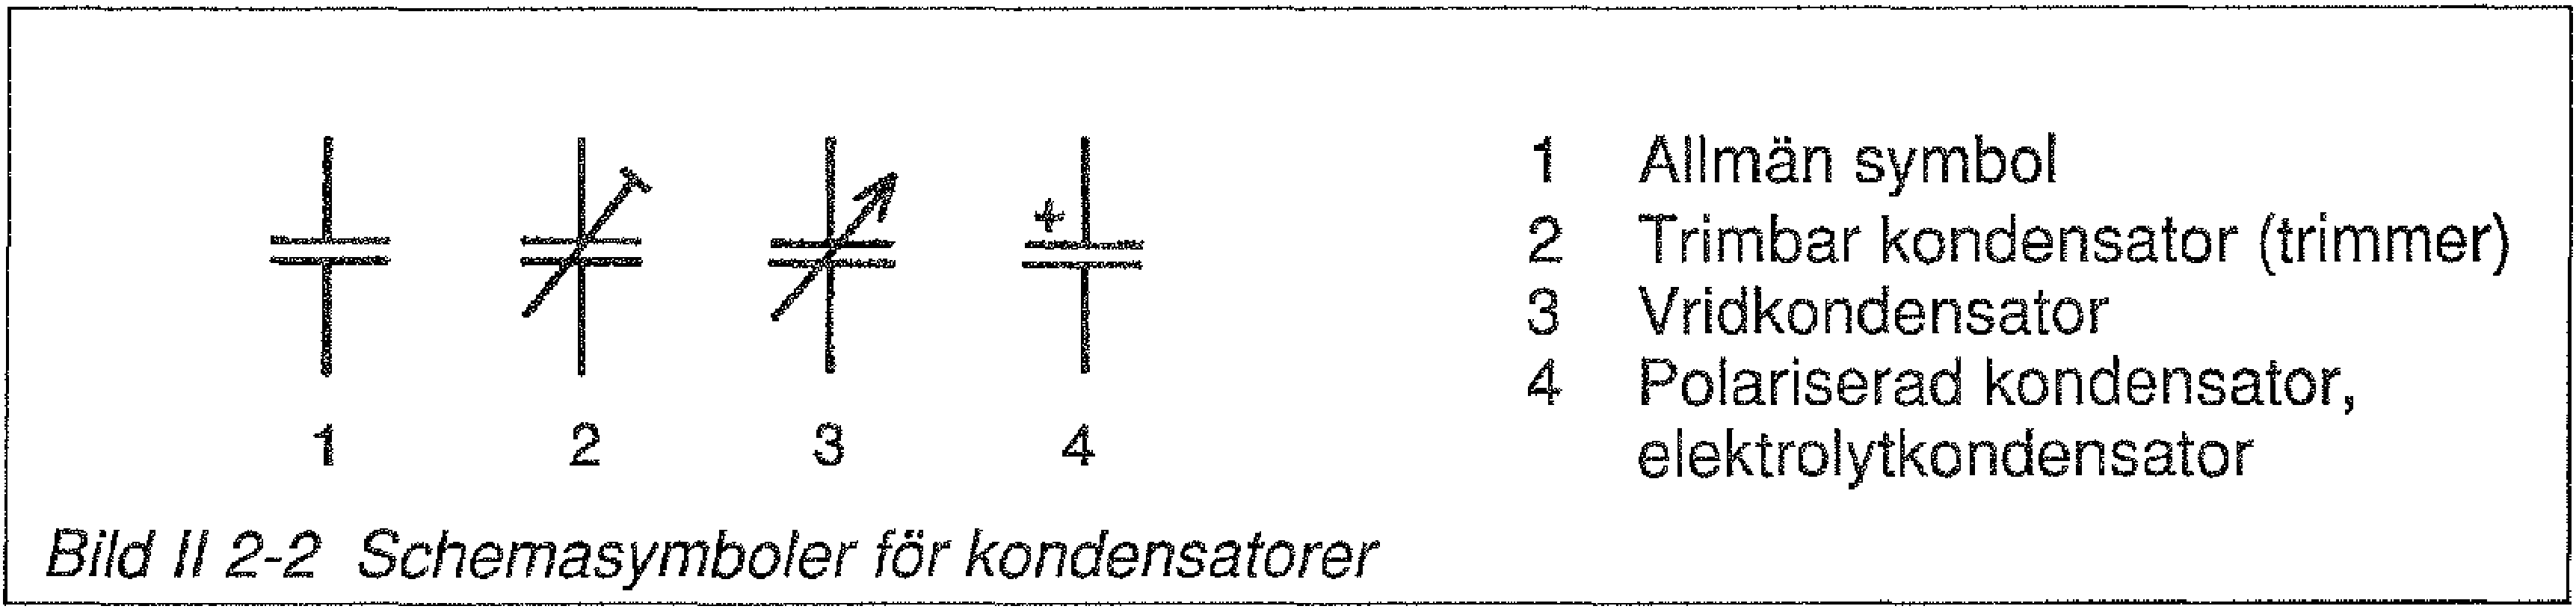
\includegraphics[width=\textwidth]{images/bild_2_2-02}
\caption{Schemasymboler för kondensatorer}
\label{fig:BildII2-2}
\end{figure}

Bild \ref{fig:BildII2-2}

Kondensatorer har oftast namn efter utförande och materialet i dielektrikum.

\emph{Pappers- och plastkondensatorer}

``Plattorna'' i dessa typer består av aluminiumremsor med anslutningstrådar.
Däremellan finns en pappers- respektive plastremsa som dielektrikum. För att
spara plats, så rullas det hela ihop och skyddas med en plastingjutning.

\emph{Keramiska kondensatorer}

I keramiska kondensatorer består dielektrikum av något keramiskt material. På
ömse sidor om detta sätts en metallbeläggning med anslutningstrådar.

\emph{Glimmerkondensatorer}

I denna kondensatortyp består dielektrikum av tunna glimmerskivor.

\emph{Elektrolytkondensatorer}

Elektrolytkondensatorer har elektroder av aluminium eller tantal, där pluspolen
(anoden) ges ett mycket tunt oxidskikt. Detta är inte ledande och fungerar som
dielektrikum. Mellan oxidskiktet och minuspolen (katoden) läggs en elektrolyt
med låg resistivitet.

Elekrolytkondensatorer har särskilt högt kapacitansvärde. Till skillnad från
andra kondensatortyper, så är elektolytkondensatorer polariserade. Utom i ett
specialfall innebär det, att polariteten på den pålagda spänningen inte får
kastas om. Flera olika slags elektrolytkondensatorer finns, såsom våta
och torra aluminiumelektrolytkondensatorer, tantalelektrolytkondensatorer m. fl.

\subsubsection{Variabla kondensatorer}
Variabla kondensatorer har oftast sitt namn efter utförandeformen, såsom
vridkondensator och trimbar kondensator (trimmer).

\subsection{Temperaturkoefficient}

På liknande sätt som med resistorer, så påverkas kapaciteten i kondensatorer av
temperaturen. Att sambandet mellan kapacitet och temperatur är viktigt, förstås
av att temperaturkoefficienten i den frekvensbestämmande kapacitansen i en
oscillatorkrets är en av faktorerna för stabil frekvens.

Temperaturkoefficienten a anger kapacitetsändringen per grad temperaturändring.
Kapacitetsändringen blir då

\[∆C = \pm \alpha _c \cdot C_k \cdot ∆\vartheta\]

varvid \(C_k\) är kapacitetsvärdet vid den lägre temperaturen (oftast 20°C) och
\(∆\vartheta\) är temperaturändringen i grader Kelvin.
Kelvin [K] är den normerade måttenheten för absolut temperatur.
En ändring med 1 K motsvarar en ändring med 1°C.

Är \(\alpha _c\) positivt betyder det att kapaciteten ökar med ökande
temperatur.

Är \(\alpha _c\) negativt betyder det att kapaciteten minskar med ökande
temperatur.

En kondensator som är märkt med N 100 betyder
\(\alpha _c = -100 \cdot 10^{-6}\ 1/K\)

\subsection{Standardiserade komponentvärden}
\index{kondensator!standardiserade värden}

Kondensatorer tillverkas vanligen med standardiserade värden ur någon talserie.

\subsection{Märkning av kondensatorer}

Kondensatorer märks med hjälp av siffror och bokstäver eller med en färgkod så att
kondensatorns huvuddata kan avläsas.
(Se f.ö. leverantörskataloger för information om komponentdata, märkning o.s.v.)
